\section{Evaluation}\label{sec:eval}

We evaluate $\tool$ using the following research questions:
\begin{itemize}
\item \textbf{RQ1) Analysis Speed-up:} How much analysis time is reduced by
using dynamic shortcuts?
\item \textbf{RQ2) Precision Improvement:} How much analysis precision is
improved by using dynamic shortcuts?
% instead of manual modeling?
\item \textbf{RQ3) Opaque Function Coverage:} How many opaque functions are
covered only by dynamic shortcuts?
% without using manual modeling?
\end{itemize}
We selected the official 306 tests of Lodash 4
(v.4.17.20)\footnote{https://github.com/lodash/lodash/blob/4.17.20/test/test.js}
used in the examples in Section~\ref{sec:motivation} as our evaluation target.
Recent work~\cite{value-refinement,
value-partitioning} also used the tests to evaluate their techniques.
Among them, we filtered out 37 tests that use JavaScript language
features SAFE does not support such as dynamic code generation using
\njscode{Function}, getters and setters, and browser-specific features like $\jscode{__proto__}$.
Thus, we used 269 out of 306 tests for the evaluation of $\tool$.
We performed our experiments on a Ubuntu machine
equipped with 4.2GHz Quad-Core Intel Core i7 and 32GB of RAM.


\subsection{Analysis Speed-up}

\begin{figure}[t]
  \centering
  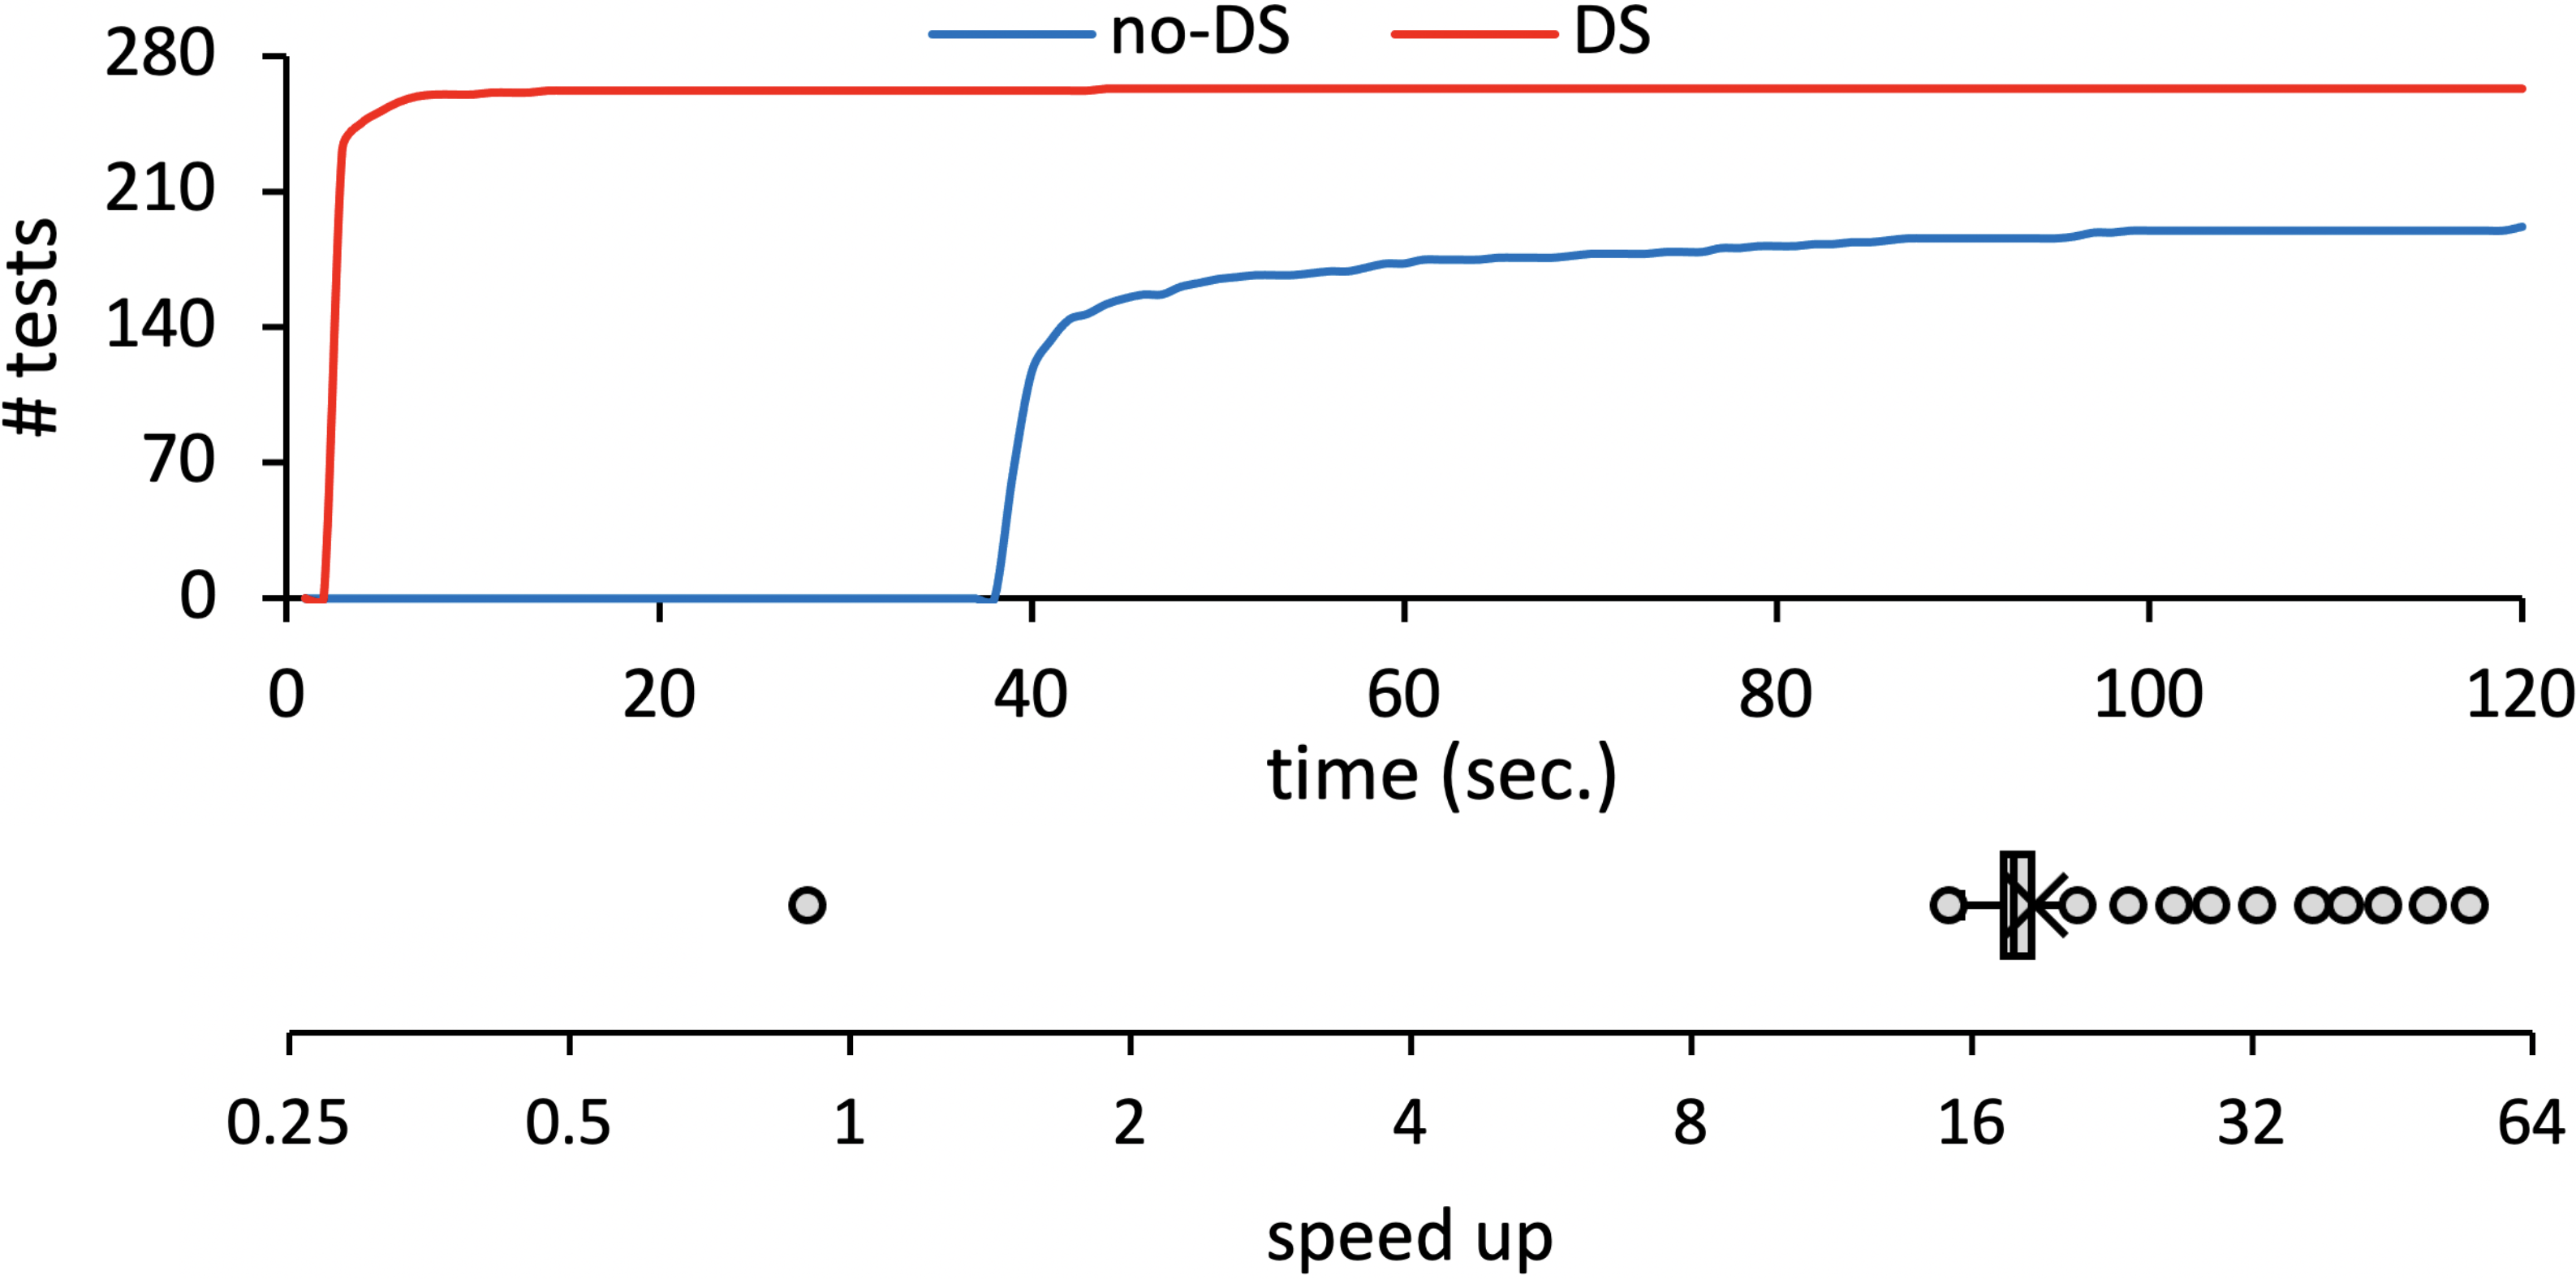
\includegraphics[width=\linewidth]{img/conc-analysis-time}
  \vspace*{-1.5em}
  \caption{Analysis time for Lodash 4 \textit{original} tests without (no-DS)
  and with (DS) dynamic shortcuts within 5 minutes}
  \label{fig:conc-analysis-time}
\vspace*{-.5em}
\end{figure}

\begin{figure}[t]
  \centering
  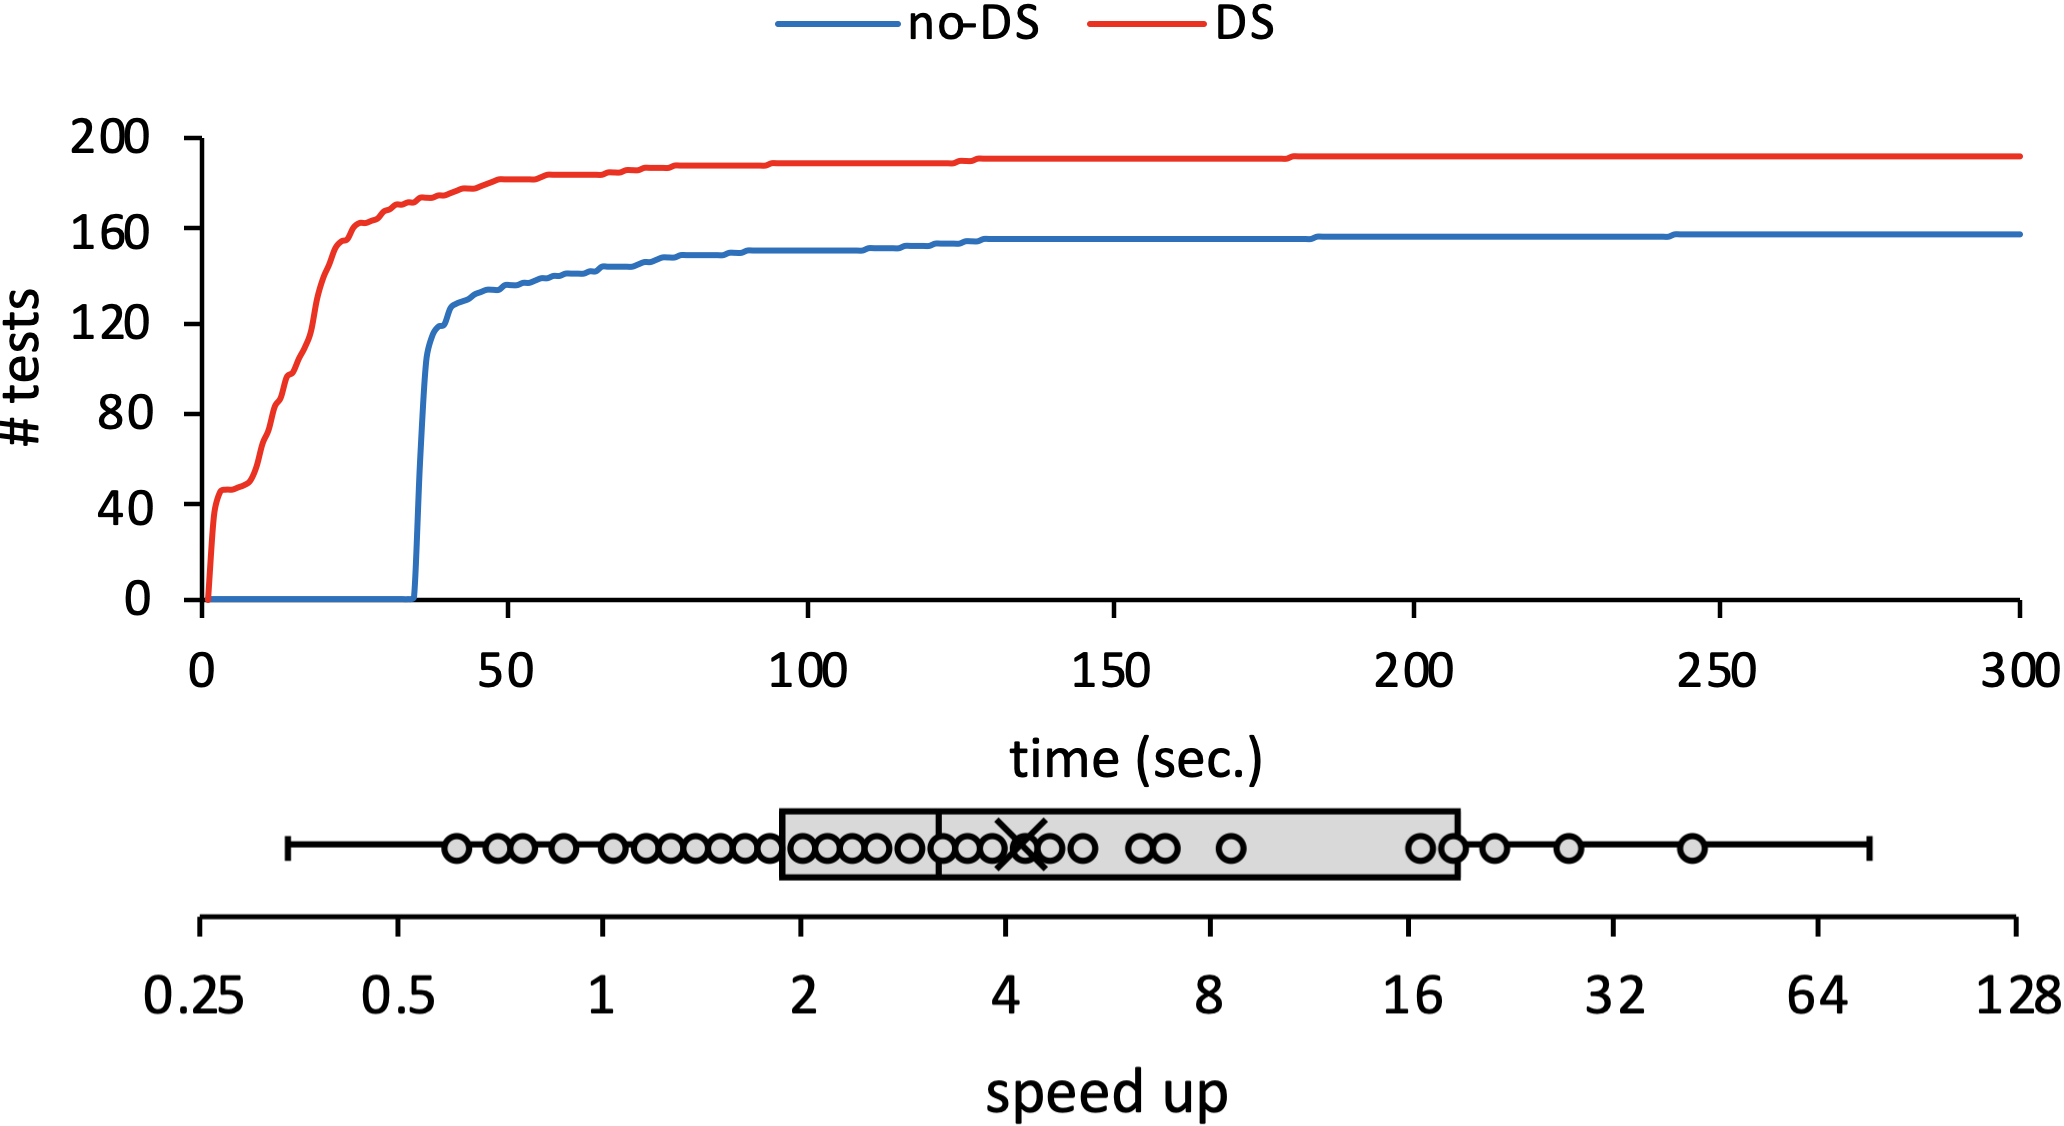
\includegraphics[width=\linewidth]{img/abs-analysis-time}
  \vspace*{-1.5em}
  \caption{Analysis time for Lodash 4 \textit{abstracted} tests without (no-DS)
  and with (DS) dynamic shortcuts within 5 minutes}
  \label{fig:abs-analysis-time}
  \vspace*{-.5em}
\end{figure}

We evaluated the effectiveness of dynamic shortcuts by static
analysis of 269 Lodash 4 tests with and without dynamic shortcuts.
%
Figure~\ref{fig:conc-analysis-time} depicts cumulative distribution charts for
their analysis time and a box plot in a logarithmic scale for speed up after
applying dynamic shortcuts.  In the upper chart, the $x$-axis is time and the
$y$-axis shows the number of tests within the time.  While the baseline analysis
(no-DS) finished analysis of 200 out of 269 tests within 5 minutes, our tool
(DS) finished analysis of 265 tests using dynamic shortcuts.  For finished
tests, the average analysis time is 49.46 seconds for no-DS and 3.21 seconds for
DS.  Among 200 tests analyzed by no-DS, one test is timeout in DS, thus
199 tests are analyzable by both analyzers. For them, we depict the box plot for
analysis speed up by dynamic shortcuts.  It shows that DS
outperforms no-DS up to 83.71$\x$ and 22.30$\x$ on
average.  Only for one test using $\jscode{_.sample}$, which
randomly samples a value from a given array, DS showed
0.36$\x$ speed of no-DS due to 24 times uses of dynamic shortcuts.

Note that since most tests use concrete values instead of
non-deterministic inputs, they can be analyzed by a few number of dynamic shortcuts.
In fact, among 269 tests, 259 tests are analyzed
by a single dynamic shortcut without using abstract semantics.
However, in real-world JavaScript programs, arguments of library
functions may include non-deterministic inputs.
To evaluate $\tool$ in a real-world setting,
we modified the tests to use abstract values.
We made abstract values by randomly selecting literals and replacing
one of them with its corresponding abstract value.
For example, if we select a numeric literal \jscode{42}, we modified it to the abstract numeric value
$\top_{\code{num}}$, which represents all the numeric values.
In the remaining section, we evaluated $\tool$ using the \textit{original} tests
and the \textit{abstracted} tests.

For abstracted tests as well, DS outperformed no-DS.
Figure~\ref{fig:abs-analysis-time} shows the analysis time of the abstracted tests.
Among 269 abstracted tests, no-DS finished analysis of 158 tests within 5 minutes,
but DS finished analysis of 193 tests.  For finished tests, the average analysis
time is 44.88 seconds for no-DS and 19.05 seconds for DS. Among 158 tests analyzed by no-DS, DS
timed-out for 2 tests.  For 156 tests analyzable by both analyzers,
DS outperformed no-DS up to 78.07$\x$ and 7.81$\x$ on average.
Except for 9 test cases, using dynamic shortcuts did show speed-ups.

\begin{figure}[t]
  \centering
  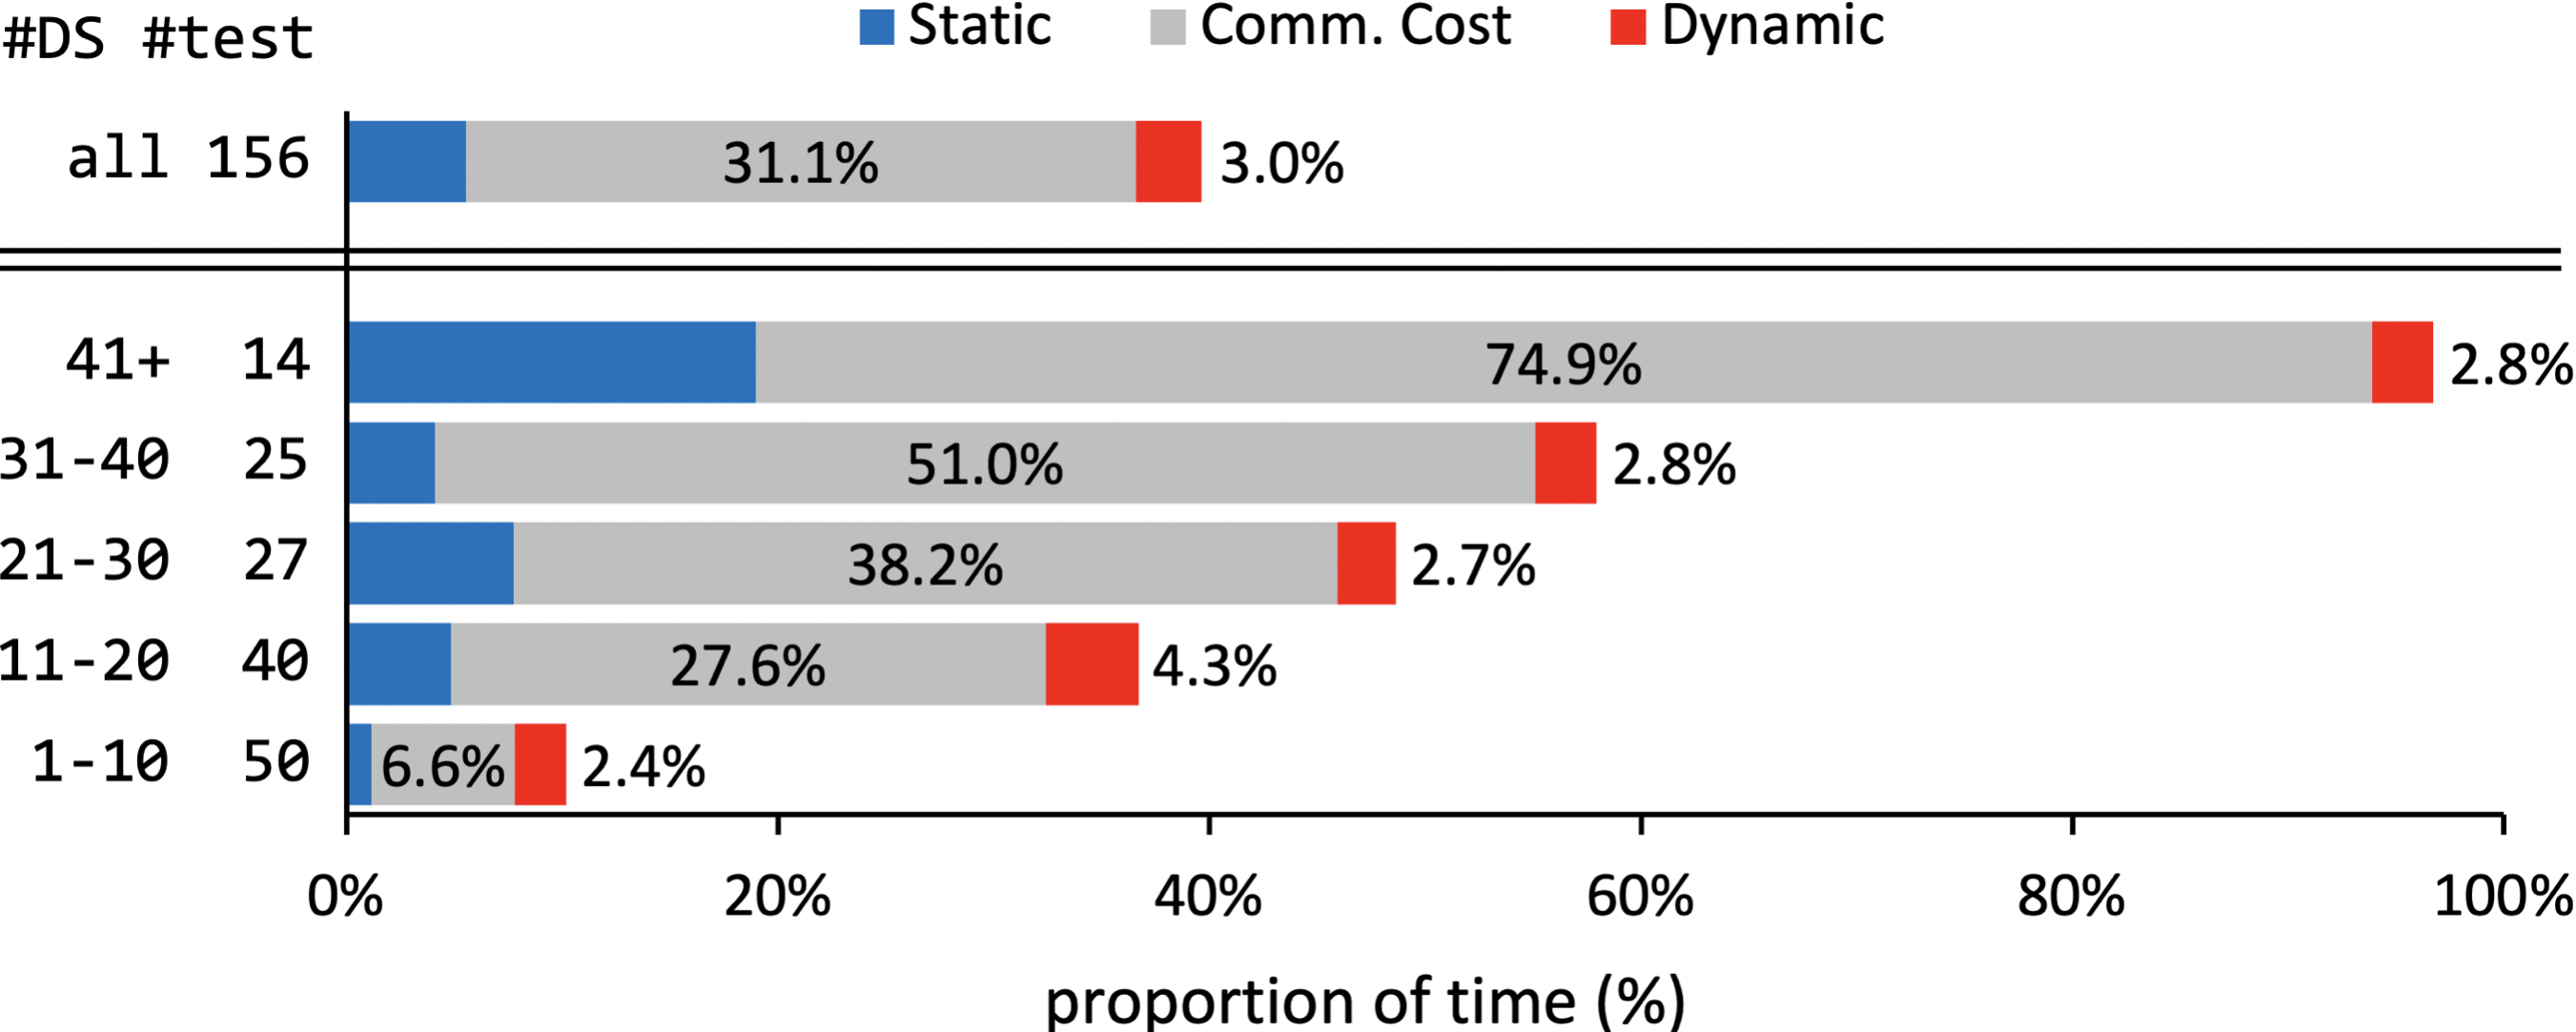
\includegraphics[width=\linewidth]{img/abs-analysis-ratio}
  \vspace*{-1.5em}
  \caption{Analysis time ratio for 156 \textit{abstracted} tests}
  \label{fig:abs-analysis-ratio}
  \vspace*{-1.5em}
\end{figure}

Unlike for the original tests, analysis of 156 abstracted tests invoked
20.35 dynamic shortcuts.  Because taking a dynamic shortcut
requires conversion between abstract states and {\sealed} values
and their exchanges between the static analyzer and the dynamic analyzer,
using dynamic shortcuts multiple times may incur more performance
overhead than performance benefits by using {\sealed} execution.
One conjecture is that the communication cost between the static
analyzer and the dynamic analyzer may be proportional to the number of
dynamic shortcuts.

To experimentally evaluate the conjecture, we investigated the relationship between
the communication cost (Comm. Cost) between analyzers and the number of dynamic shortcuts.
For 199 original tests, Comm. Cost was only
1.58\% compared to the analysis time of no-DS.  However, for 156
abstracted tests, Comm. Cost was 31.06\% compared to the analysis
time of no-DS.  Figure~\ref{fig:abs-analysis-ratio} presents the
analysis time ratio for 156 abstracted tests.
The $x$-axis represents the time ratio normalized by the total analysis time of
no-DS and the $y$-axis denotes the number of dynamic
shortcuts and the number of corresponding tests.
For all 156 tests, Comm. Cost is larger than
both the static analysis time (Static) and the dynamic analysis
time (Dynamic).  When dynamic shortcuts are performed less than 10 times,
Comm. Cost is modest compared to the baseline static
analysis time.  However, the more dynamic shortcuts are performed,
the less the performance benefits by using dynamic shortcuts.
Specifically, when dynamic shortcuts are performed more than 30 times,
Comm. Cost is even larger than half of cost of no-DS.
Based on this evaluation result, we believe that we can leverage
dynamic shortcuts by optimizing Comm. Cost between
the static analyzer and the dynamic analyzer.

\begin{figure}[t]
  \centering
  \begin{subfigure}[t]{0.23\textwidth}
    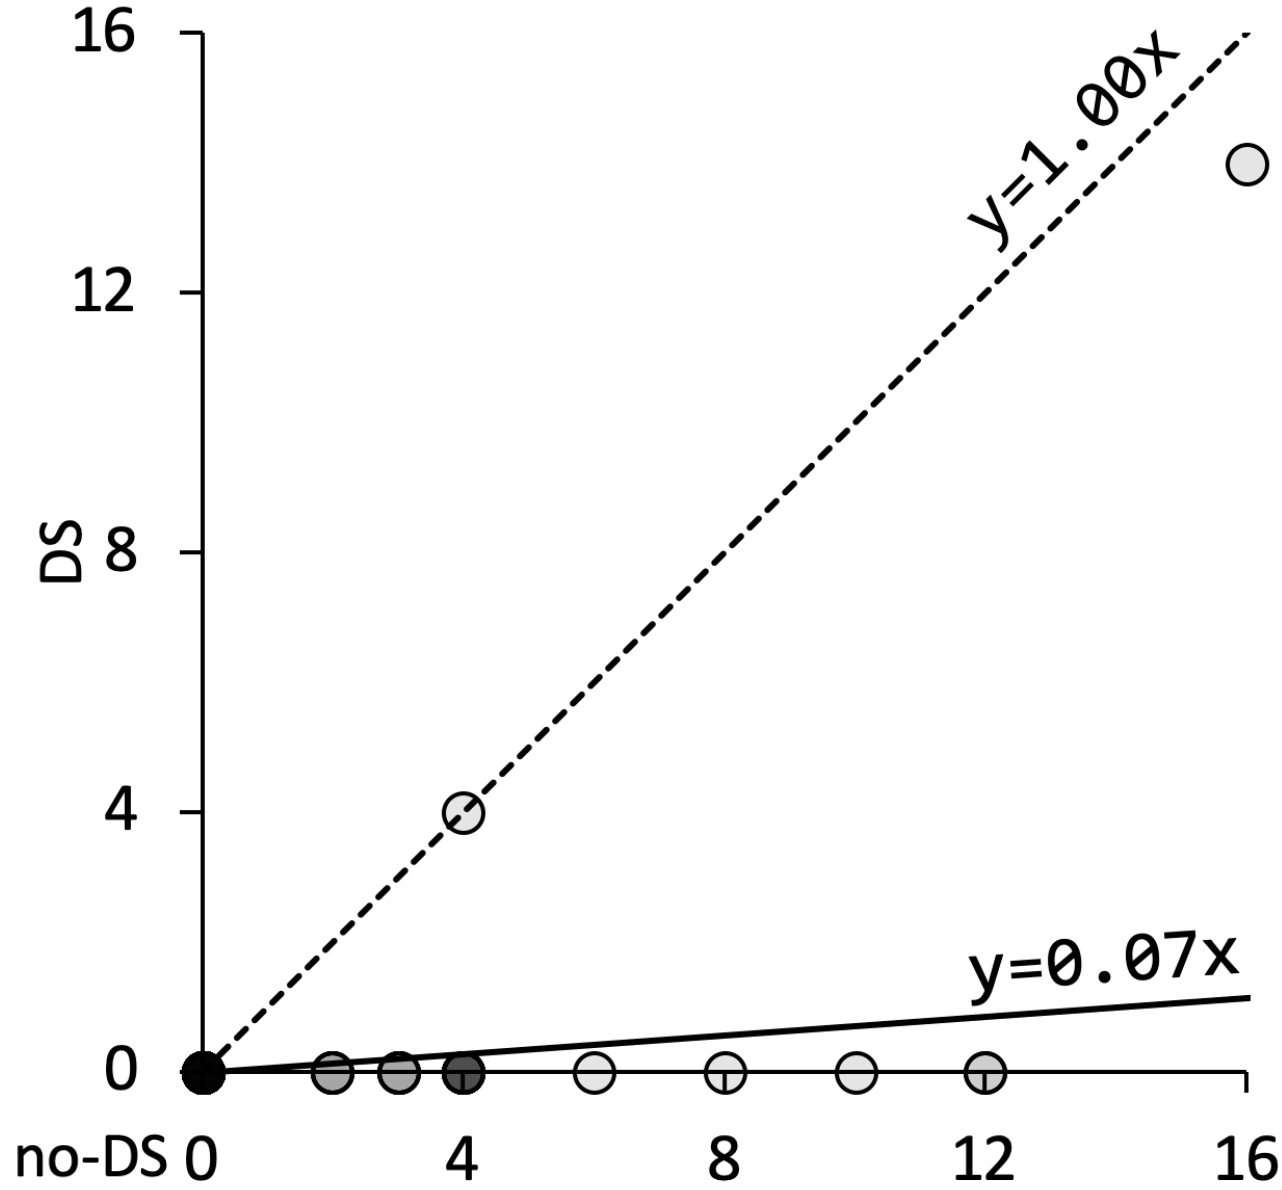
\includegraphics[height=3.2cm]{img/conc-precision}
    \vspace*{-0.7em}
    \caption{199 \textit{original} tests}
    \label{fig:conc-precision}
  \end{subfigure}
  \begin{subfigure}[t]{0.23\textwidth}
    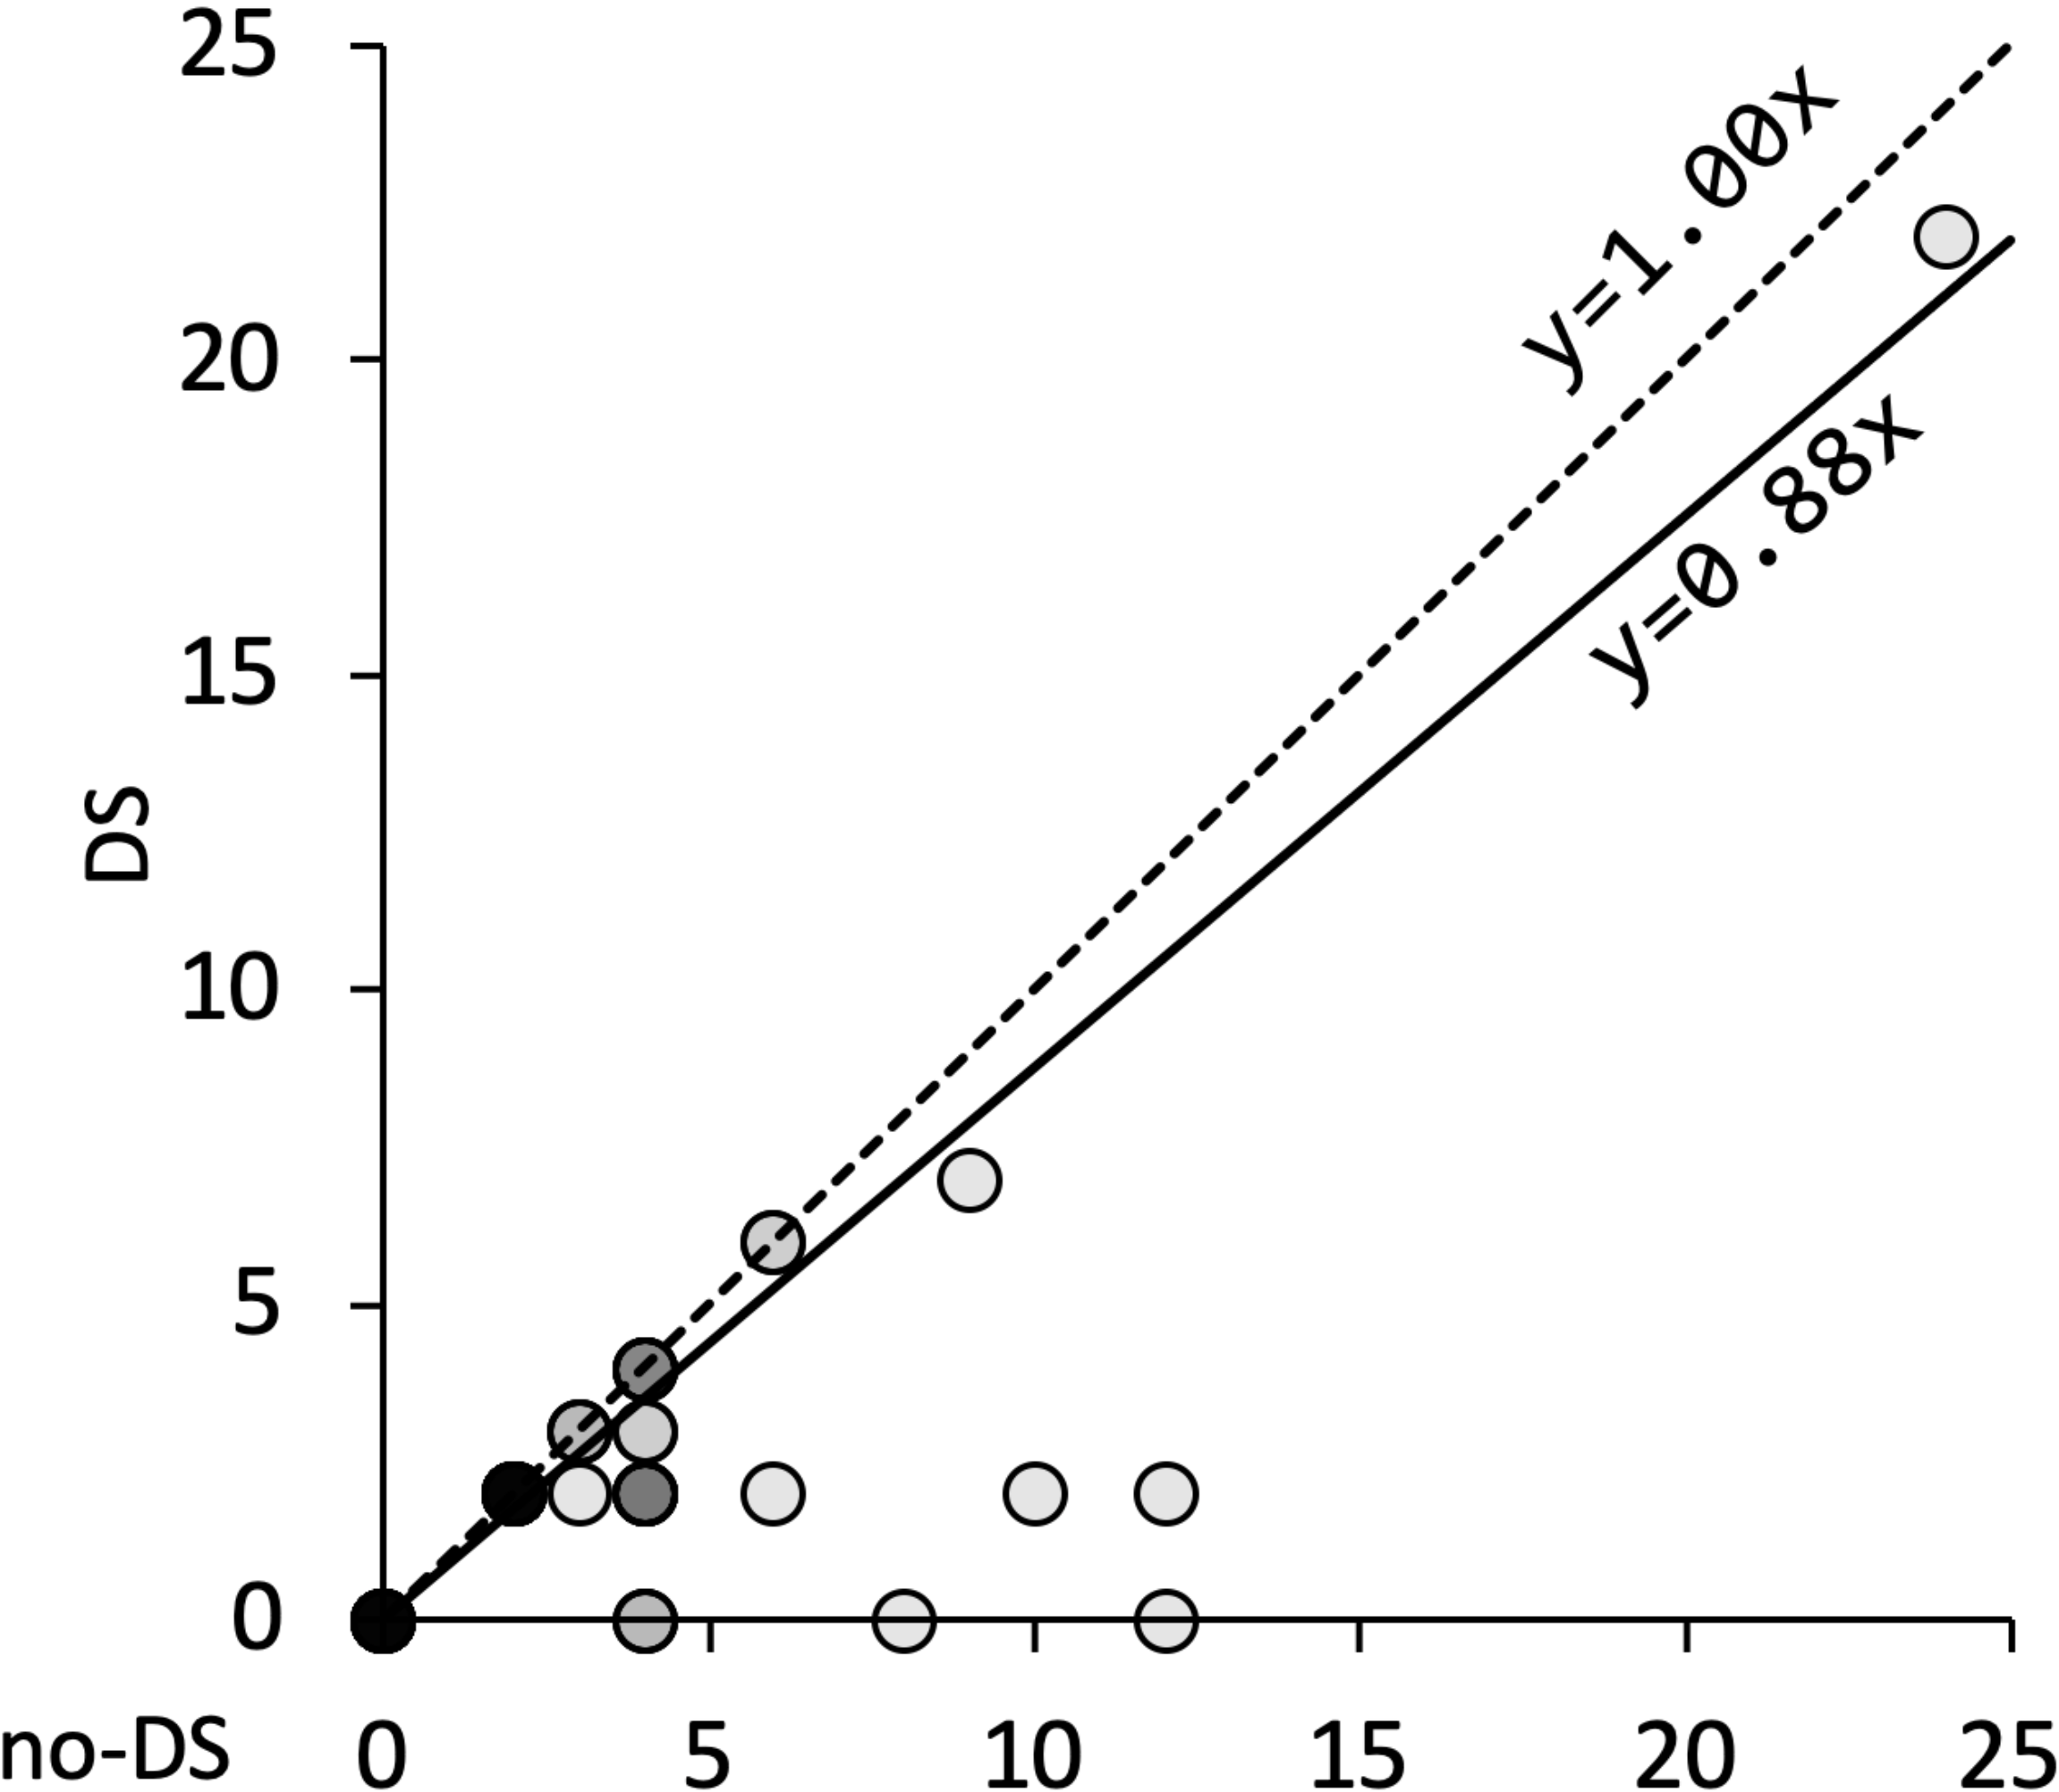
\includegraphics[height=3.2cm]{img/abs-precision}
    \vspace*{-0.7em}
    \caption{156 \textit{abstracted} tests}
    \label{fig:abs-precision}
  \end{subfigure}
  \vspace*{-1em}
  \caption{Failed assertions of analysis without (no-DS) and with (DS) dynamic shortcuts}
  \label{fig:precision}
  \vspace*{-1.5em}
\end{figure}


\begin{table*}[t]
  \caption{Number of original (orig.) and abstracted (abs.) tests using dynamic shortcuts
only for each JavaScript built-in library}
  \label{table:func-replace}
  \vspace*{-1.5em}
  \centering
  \scriptsize
  \[
\quad
    \begin{array}{c|l|c|c?c|l|c|c?c|l|c|c}

      \myhead{Object}       {Function}        {\# Replaced}

      \mysuff{1}{}          {Array    }  {204 / 205}{119 / 141} 	& \mysutf{1}{}             {String     }  { 20 /  20}{ 13 /  14} 	& \mysutf{1}{}       {Object        }  {265 / 265}{181 / 193} \mylinefff
      \mysuff{1}{}          {new Array}  {  0 /   0}{  0 /   7} 	& \mysuff{1}{}             {toString   }  {  0 /   0}{  0 /  14} 	& \mysutf{1}{}       {getPrototypeOf}  { 56 /  56}{ 34 /  35} \mylinefff
      \mysuff{1}{}          {isArray  }  {264 / 265}{181 / 193} 	& \mysuff{1}{}             {valueOf    }  {  0 /   0}{  0 /  20} 	& \mysbtt{1}{}       {create        }  {265 / 265}{193 / 193} \mylinefff
      \mysutf{1}{}          {concat   }  {265 / 265}{189 / 193} 	& \mysutt{1}{}             {charAt     }  {  8 /   8}{  6 /   6} 	& \mysutf{2}{Object} {defineProperty}  {265 / 265}{190 / 193} \mylinefff
      \mysutt{1}{}          {join     }  {265 / 265}{193 / 193} 	& \mysutt{1}{}             {charCodeAt }  { 15 /  15}{  8 /   8} 	& \mysbtt{1}{}       {freeze        }  {  1 /   1}{  1 /   1} \mylinefff
      \mysutt{1}{}          {pop      }  { 25 /  25}{ 14 /  14} 	& \mysutt{1}{}             {indexOf    }  {  2 /   2}{  1 /   1} 	& \mysutf{1}{}       {keys          }  {265 / 265}{191 / 193} \mylinefff
      \mysutf{2}{Array}     {push     }  {265 / 265}{186 / 193} 	& \mysutf{2}{String}       {match      }  { 26 /  26}{ 16 /  18} 	& \mysuff{1}{}       {toString      }  {264 / 265}{138 / 193} \mylinefff
      \mysutt{1}{}          {reverse  }  { 10 /  10}{  6 /   6} 	& \mysutf{1}{}             {replace    }  { 56 /  56}{ 31 /  37} 	& \mysutf{1}{}       {hasOwnProperty}  {265 / 265}{190 / 193} \mylinefft
      \mysutt{1}{}          {shift    }  {  3 /   3}{  2 /   2} 	& \mysutf{1}{}             {slice      }  {265 / 265}{191 / 193} 	& \mysbtt{1}{JSON}   {stringify}       {  1 /   1}{  1 /   1} \mylinefft
      \mysutt{1}{}          {slice    }  {265 / 265}{193 / 193} 	& \mysutt{1}{}             {split      }  {  5 /   5}{  2 /   2} 	& \mysutf{1}{}       {parseInt}        {  2 /   2}{  1 /   2} \mylinefff
      \mysutf{1}{}          {sort     }  { 69 /  69}{ 38 /  39} 	& \mysutf{1}{}             {substring  }  {214 / 214}{136 / 145} 	& \mysutf{1}{Global} {isNaN   }        { 15 /  15}{ 11 /  40} \mylinefff
      \mysutf{1}{}          {splice   }  { 25 /  25}{  9 /  12} 	& \mysutf{1}{}             {toLowerCase}  {215 / 215}{135 / 146} 	& \mysbtt{1}{}       {isFinite}        {  3 /   3}{  1 /   1} \mylinefft
      \mysutt{1}{}          {unshift  }  {  2 /   2}{  2 /   2} 	& \mysutf{1}{}             {toUpperCase}  { 11 /  11}{  6 /   7} 	& \mysbtt{1}{}       {RegExp    }      {265 / 265}{193 / 193} \mylinefff
      \mysutf{1}{}          {indexOf  }  { 94 /  94}{ 61 /  66} 	& \mysutt{1}{}             {fromCharCode} {  1 /   1}{  1 /   1}  &	\mysuff{2}{RegExp} {new RegExp}      {  0 /   0}{  0 /   1} \mylineftf
      \mysutf{1}{}          {every    }  { 92 /  92}{ 43 /  47} 	& \mysuff{1}{Date}         {new Date}     {  0 /   1}{  0 /   1} 	& \mysbtt{1}{}       {exec      }      {265 / 265}{193 / 193} \mylinettf
      \mysuff{1}{}          {ceil }      { 37 /  38}{ 20 /  21} 	& \mysutt{1}{}             {Number}       {  2 /   2}{  2 /   2} 	& \mysuff{1}{}       {test      }      {264 / 265}{185 / 193} \mylinefft
      \mysuff{1}{}          {floor}      { 16 /  18}{  8 /  10} 	& \mysutf{1}{Number}       {toFixed}      {  1 /   1}{  0 /   0} 	& \mysutf{1}{}       {Error     }      {  1 /   1}{  0 /   1} \mylinefff
      \mysuff{2}{Math}      {max  }      {264 / 265}{179 / 193} 	& \mysuff{1}{}             {valueOf}      {  0 /   0}{  0 /  28} 	& \mysuff{1}{Error}  {new RangeError}  {  0 /   0}{  0 /   2} \mylineftf
      \mysutf{1}{}          {min  }      { 64 /  64}{ 31 /  44} 	& \mysutt{1}{}             {toString}     {265 / 265}{193 / 193} 	& \mysuff{1}{}       {new TypeError }  {  0 /   0}{  0 /   7} \mylinefft
      \mysutt{1}{}          {pow  }      { 11 /  11}{  6 /   6} 	& \mysuff{1}{Function}     {apply   }     {263 / 265}{133 / 193} 	& \mysbtt{2}{Boolean}{Boolean}         {  3 /   3}{  2 /   2} \mylinefff
      \mysutt{1}{}          {round}      {  2 /   2}{  1 /   1} 	& \mysuff{1}{}             {call    }     {259 / 265}{ 50 / 193} 	& \mysuff{1}{}       {valueof}         {  0 /   0}{  0 /   7}
    \end{array}
  \]
  \vspace*{-1em}
\end{table*}



\subsection{Precision Improvement}

To evaluate the analysis precision improvement of dynamic shortcuts,
we measured the number of failed assertions produced by no-DS and DS.
Because both no-DS and DS are sound,
high (low) number of failed assertions denotes low (high) analysis precision.

Figure~\ref{fig:precision} depicts the comparison of the analysis
precision between no-DS and DS.  The $x$-axis and the $y$-axis denote
the number of failed assertions produced by no-DS and DS, respectively;
each circle denotes each test in the heat-map form. The darker the circle is, the more tests it indicates.
The top line
denotes the y=x line, and the bottom solid line denotes the average improvement.
For 199 original tests that are analyzable by both analyzers,
Figure~\ref{fig:precision}(a) shows that dynamic shortcuts
completely removed the failed assertions for 24 tests, reducing the number of failed assertions by 92.79\% on average.
For 156 abstracted tests that are analyzable by both analyzers,
Figure~\ref{fig:precision}(b) shows that dynamic shortcuts successfully cut down
the number of failed assertions by 12.31\% on average.
Thus, on average, dynamic shortcuts removed analysis of 92.79\% and 12.31\% failed assertions
for original and abstracted tests, respectively.
